\section{Platform Design}\label{sec:approach}

In this section, we outline the guiding principles behind the current platform architecture. 
In order to precisely identify the main application scenarios and objectives, a thorough requirement gathering phase has been carried out taking into account the first principles underpinning Big Data solutions and the expectations of the business partners involved in the project. The main requirements drove the core design of the platform. As the platform deals with issues of data processing, integration, enrichment, and extension, it needed to support data flow definition and execution. 
Furthermore, EW-Shopp business cases provided input data sets in tabular format from heterogeneous domains, and of different volumes, including Big Data. In many cases, the data provided by organizations was a core asset and thus, also data confidentiality needed to be retained. 
Due to the varying security requirements of organizations, the system had to be designed to flexibly support different security setups. The data flows themselves had to be defined on a high level and composed of independent steps, which also include data integration and enrichment at scale. Finally, deployment of the flows had to be flexible in terms of both hardware and software, so that they can be deployed in different infrastructures that fit organizational needs best.
The main specific platforms for data wrangling available on the market have been also evaluated, and in particular, OpenRefine\footnote{\url{http://openrefine.org/}}, Trifacta Wrangler\footnote{\url{https://www.trifacta.com/products/wrangler/}} and Karma\footnote{\url{http://usc-isi-i2.github.io/karma/}}. 

At the end of this process, the need for an \textit{open source} platform, capable of managing data in \textit{tabular format} and of generating \textit{linked data}, became clear. 
In addition, two possible use cases have emerged. In the first case, small amounts of data have to be manipulated, the platform has to be lean and \textit{easy to install on a commodity machine} similarly to tools like OpenRefine. In the second scenario a genuinely big data must be managed, this means that a domain expert user must be able to describe the transformation through a user-friendly and interactive interface and to execute it in an automated way as a \textit{batch} process (as in Karma and Trifacta Wrangler). 
Common to both scenarios is the need to supply linking and enrichment services to manage \textit{geocoding}, \textit{schema linking}, \textit{entity linking} and extension with \textit{weather} and \textit{events} data. 

In an attempt to give a syncretic response to the needs outlined in the requirements, we have based platform design on two fundamental driving principles:  \textit{Separation of Concerns} and \textit{Dimension Reduction}.  
In particular, by applying separation of concerns, we have conceived the platform as composed of three tiers (Figure~\ref{fig:architecture}):

\begin{description}
    \item[Core Data Services] (in light blue): These components provide access to corporate on-boarding or third party data. These data sets are used in both data linking and extension processes. Figure~\ref{fig:architecture} shows services to access the project's core data, i.e., weather (W), events (E) and Products (P). Other enrichment sources may include services as Wikifier\footnote{\url{http://wikifier.org/}}, and freely accessible knowledge bases such as DBpedia\footnote{\url{https://wiki.dbpedia.org/}}.
    \item[Platform Services] (in green): data preparation, analytics and visualization services (the last two are not addressed in this paper). These services offer simple and intuitive user interfaces for creating (and executing if the working table is small enough) data wrangling, linking and extension pipelines.
    \item[Corporate Services] (in red): These services implement platform components needed for data governance, i.e., ingestion, storage, processing, data flow and security management of massive data sets. This tier is used to perform data wrangling operations at scale. 
\end{description}


The rationale of the Dimension Reduction~\cite{rojas2017sampling, ur2016big} approach in Big Data is also rather simple in its general lines; it consists in reducing the size of the data set by identifying a possible compact representation (i.e., a subset of data plus a profile). In this way, the data transformation operations can be designed and tested on set that can be several orders of magnitude smaller than the original. This should ensure greater responsiveness and efficiency for the applications involved without negatively affecting accuracy. For this reason, we have introduced into the platform a specialized component, whose task is to properly generate this data subset. 
We remark that the presented design choices do not reduce the applicability and generality of the presented architecture as, where it is possible (e.g., in cases where the data to be transformed is manageable), the corporate subsystem can be excluded. In this mode, the user can work directly against the original data set.


 
\begin{figure}[t]
\centering
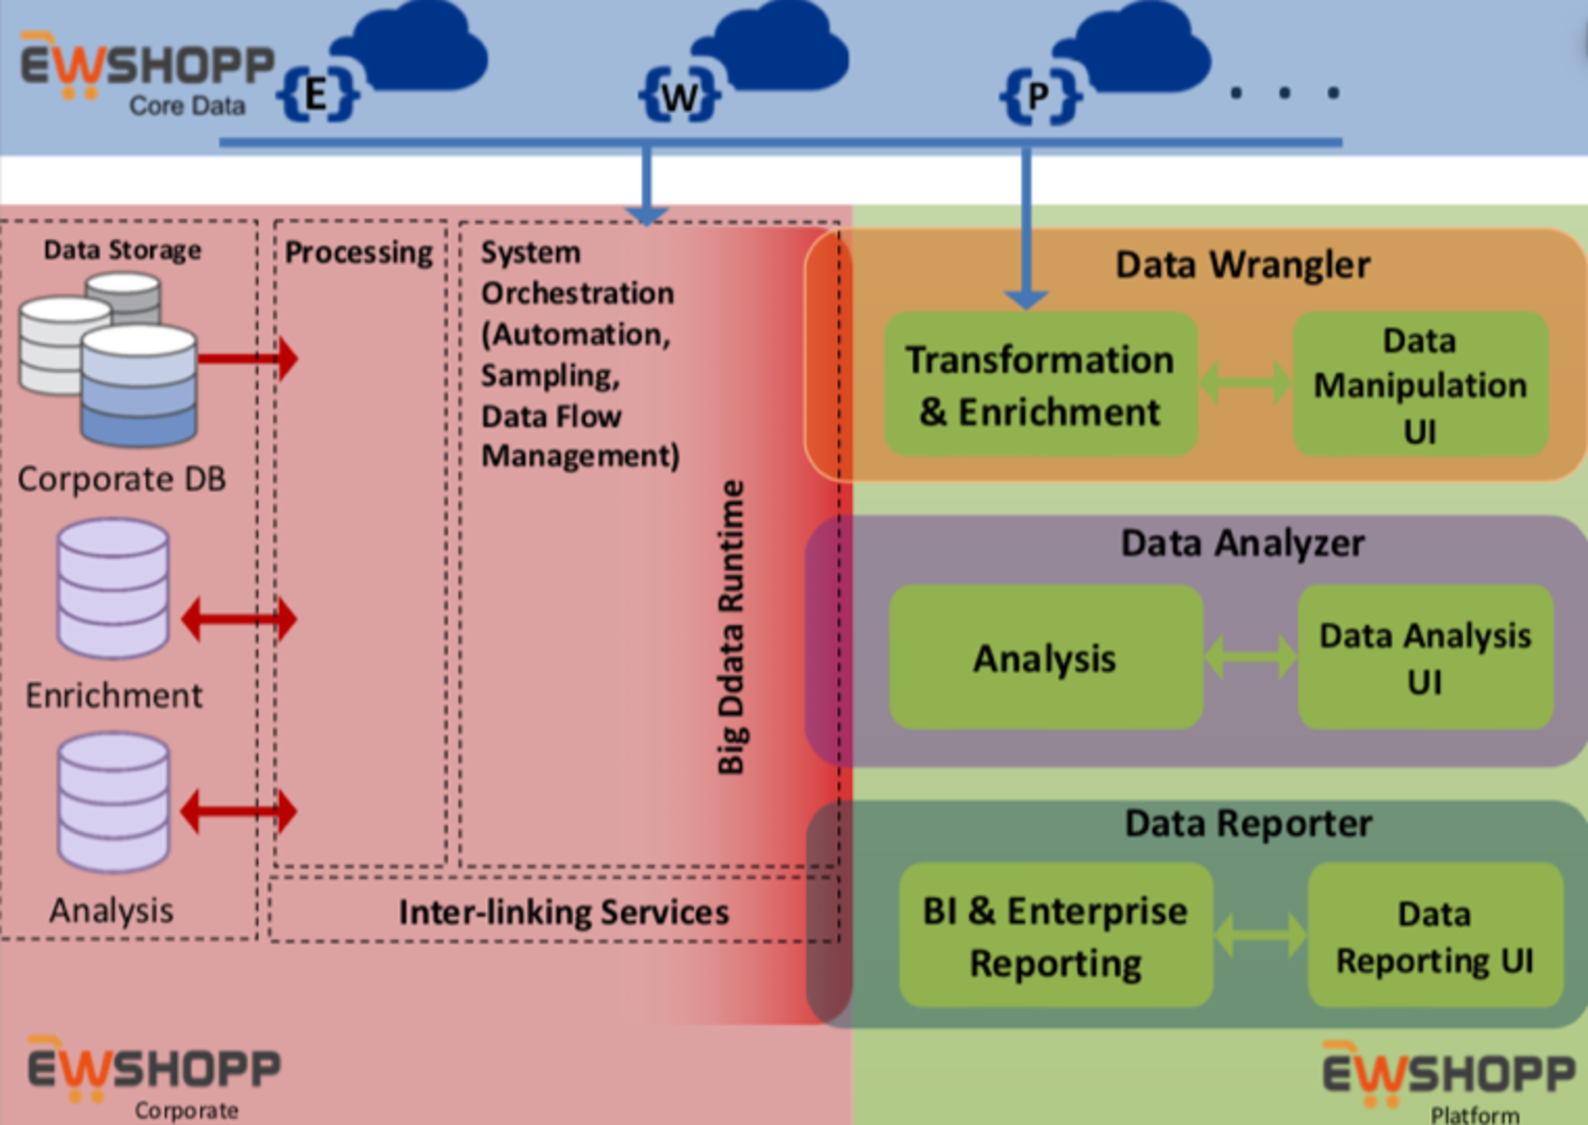
\includegraphics[width=\columnwidth]{figs/Architecture.pdf}
%\vspace{-.3cm}
\caption{General architecture}
\label{fig:architecture} 
\end{figure}  




%- open source
%- linking data
%- data onboarding https://www.trifacta.com/blog/data-onboarding-broken-matters/
%- sampling
%- backend batch execution
%- wrangling separato per essere usato cosi com'è per evitare di installare e gestire la piattaforma retrostante.
%- Servizi di interlinking e estensione
%- Gestione dei dati core del progetto. 




%The EW-Shopp system aims to support e-commerce, retail and marketing industries in improving their efficiency and competitiveness through providing the ability to perform predictive and prescriptive analytics over integrated and enriched large data sets using open and flexible solutions. 
%In addition, these tools must provide a responsive graphical user interface to guide the user in designing data transformations. 
 